% !TeX root = main.tex

\section[A4: DH Parameters]{DH Parameters of a 7R Manipulator}

\subsection*{Modified DH Parameters}

The DH Parameters are given by

\begin{enumerate}
    \item $a_{i-1}$ \emph{link length}: Distance from $Z_{i-1}$ to $Z_i$ measured along $X_{i-1}$
    \item $\alpha_{i-1}$ \emph{link twist}: Angle measured from $Z_{i-1}$ to $Z_i$ measured along $X_{i-1}$ (using right hand thumb rule)
    \item $d_i$ \emph{joint offset}: Distance from $X_{i-1}$ to $X_i$ measured along $Z_i$
    \item $\theta_i$ \emph{joint angle}: Angle measured from $X_{i-1}$ to $X_i$ measured along $Z_i$ (using right hand thumb rule)
\end{enumerate}

The transformation matrix to represent frame $\{i\}$ in frame $\{i-1\}$ is given by

\begin{equation}
    _{i}^{i-1}\mathbf{T} = \begin{bmatrix}
        \cos(\theta_i) & -\sin(\theta_i) & 0 & a_{i-1} \\
        \cos(\alpha_{i-1}) \sin(\theta_i) & \cos(\alpha_{i-1}) \cos(\theta) & -\sin(\alpha_{i-1}) & -d_i \sin(\alpha_{i-1}) \\
        \sin(\alpha_{i-1}) \sin(\theta_i) & \sin(\alpha_{i-1}) \cos(\theta) & \cos(\alpha_{i-1}) & d_i \cos(\alpha_{i-1}) \\
        0 & 0 & 0 & 1
        \end{bmatrix}
    \label{eq:dh-tf-matrix}
\end{equation}

We use Equation \ref{eq:dh-tf-matrix} to construct transformation matrices from DH parameters

% TODO: Work from here
\subsection[A4.1: 7R DH Parameters]{DH Parameters of a 7R Robot}

The given robot is a \href{https://www.kuka.com/en-in/products/robotics-systems/industrial-robots/lbr-iiwa}{KUKA LBR iiwa} collaborative robot.

\begin{figure}[ht]
    \centering
    \begin{subfigure}[b]{0.9\textwidth}
        \centering
        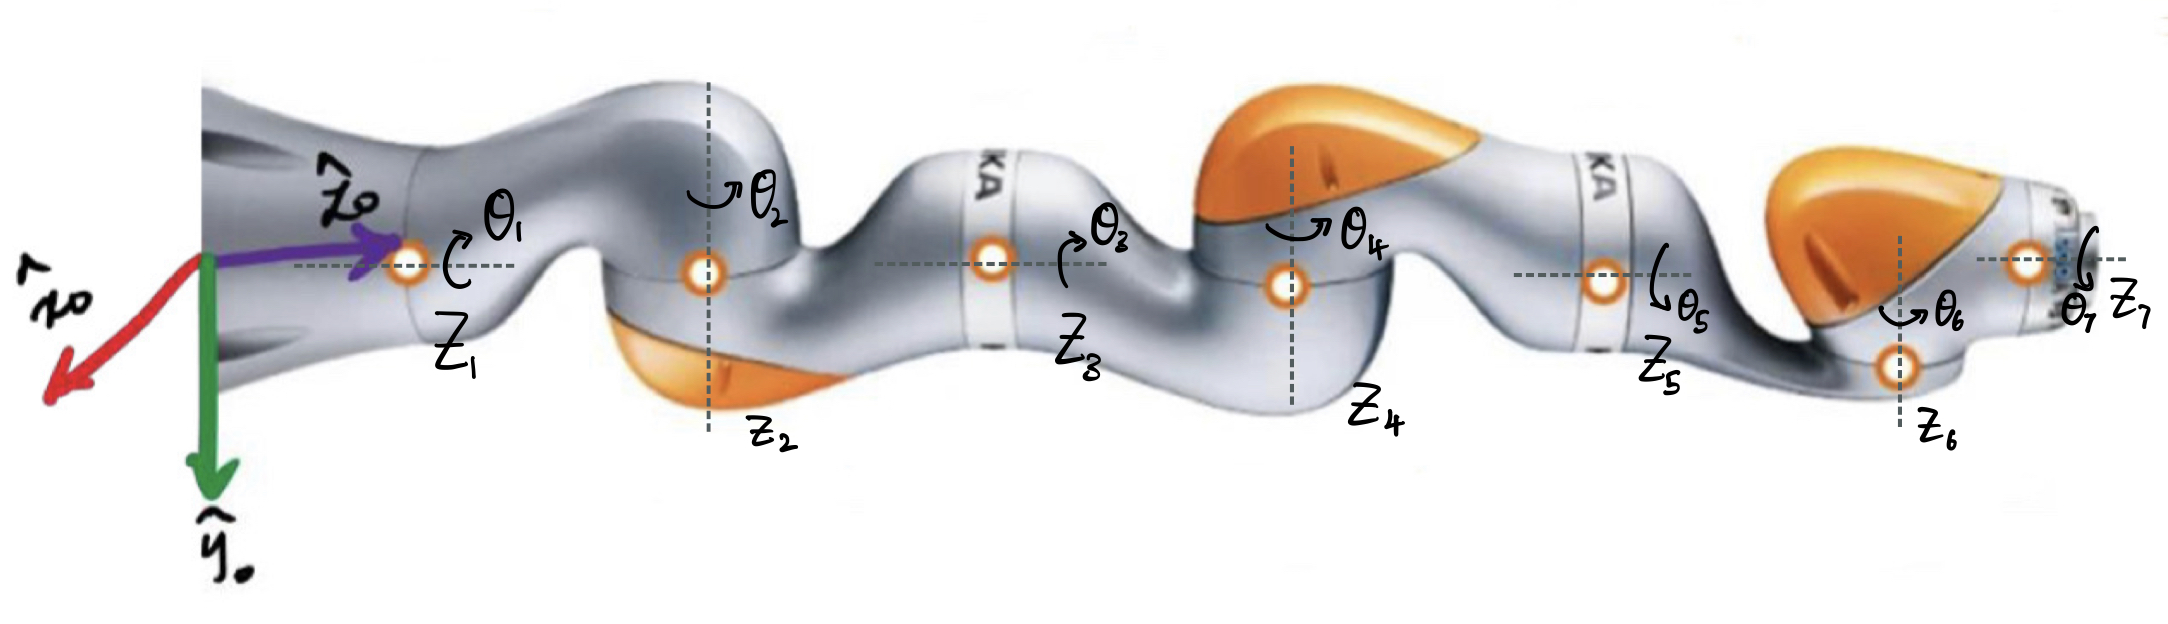
\includegraphics[width=\textwidth]{e4-7r-axis.jpg}
        \caption{Axis}
        \label{fig:sfig-7r-axis}
    \end{subfigure}
    \begin{subfigure}[b]{0.9\textwidth}
        \centering
        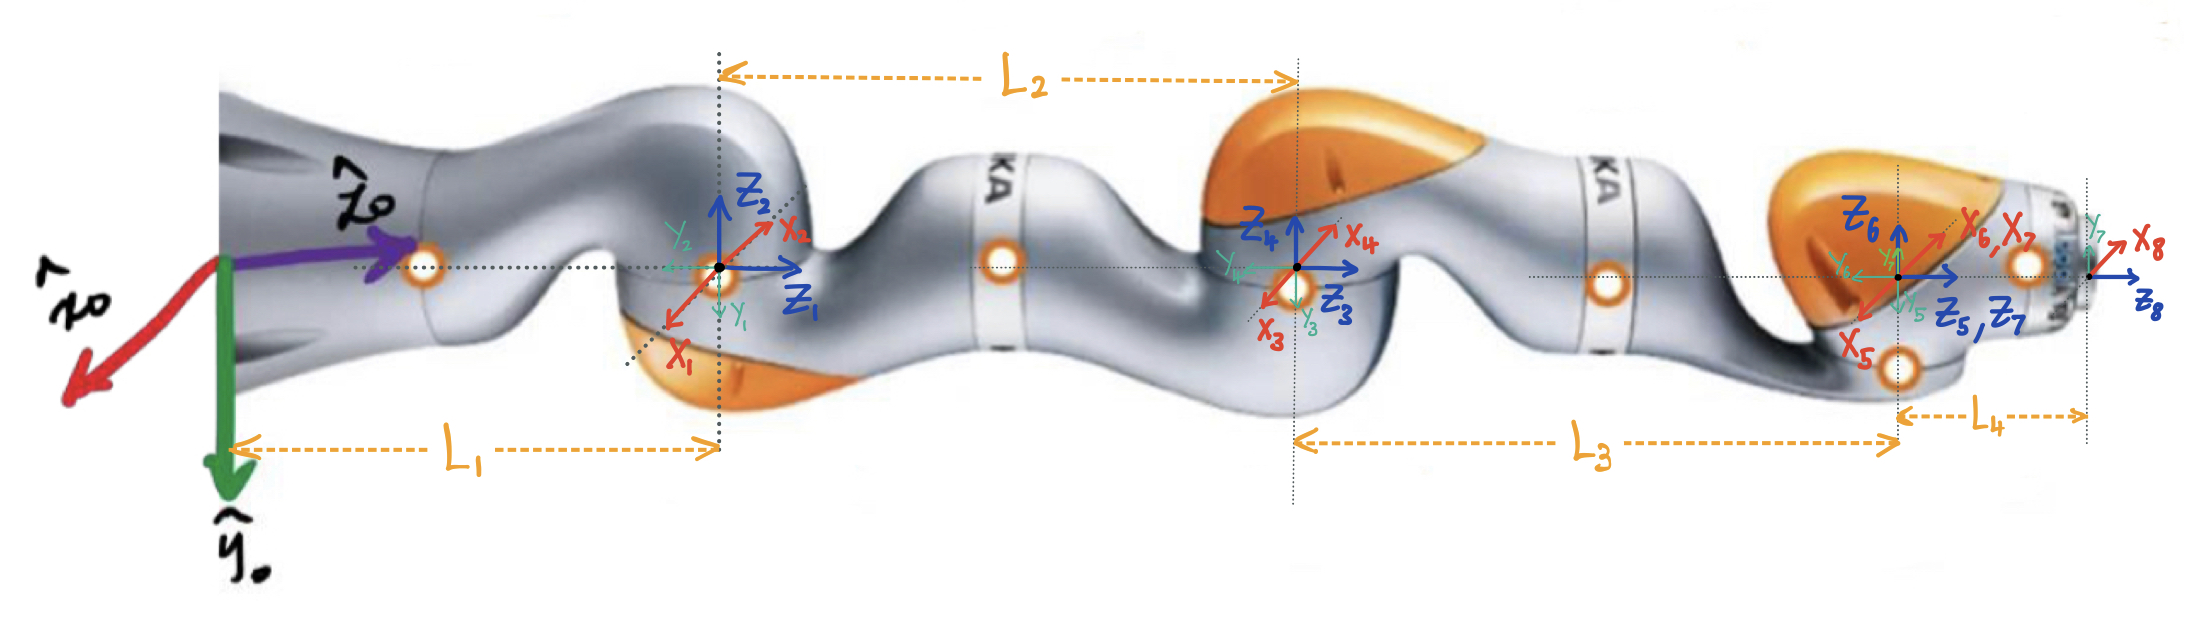
\includegraphics[width=\textwidth]{e4-7r-dh-axis.jpg}
        \caption{Frames}
        \label{fig:sfig-7r-dh-frames}
    \end{subfigure}
    \caption{Frames and Axis of given 7R robot}
    \label{fig:7r-frames}
    \small
        In sub-figure \ref{sub@fig:sfig-7r-axis}, the axis of joints are shown. In sub-figure \ref{sub@fig:sfig-7r-dh-frames}, the frames (assigned according to modified DH convention) are shown. Only the \textcolor{blue}{Z axis} and \textcolor{red}{X axis} are emphasized (as \textcolor{green}{Y axis} can be deduced using $Y = Z \times X$). In the home configuration, it is assumed that there is no vertical offset in the axis that are aligned horizontally (all origins are colinear).
\end{figure}


The axis of rotations (joint axis), and the frames are given in Figure \ref{fig:7r-frames}. The DH Parameters of the 7R robot is mentioned in Table \ref{tab:7r-dh-params}.

\begin{table}[ht]
    \centering
    \begin{tabular}{ ||c|c|c|c|c|| }
        \hline\hline
        \textbf{i} & $a_{i-1}$ & $\alpha_{i-1}$ & $d_i$ & $\theta_i$ \\
        \hline
        1 & 0 & 0 & $L_1$ & $\theta_1$ \\
        2 & 0 & $\pi/2$ & 0 & $\pi + \theta_2$ \\
        3 & 0 & $\pi/2$ & $L_2$ & $\pi+\theta_3$ \\
        4 & 0 & $\pi/2$ & 0 & $\pi + \theta_4$ \\
        5 & 0 & $\pi/2$ & $L_3$ & $\pi + \theta_5$ \\
        6 & 0 & $\pi/2$ & 0 & $\pi + \theta_6$ \\
        7 & 0 & $\pi/2$ & 0 & $\theta_7$ \\
        8 & 0 & 0 & $L_4$ & 0 \\
        \hline\hline
    \end{tabular}
    \caption{\label{tab:7r-dh-params}Table of DH Parameters for 7R}
    \small
        These are the DH Parameters for the manipulator given in Figure \ref{fig:7r-frames}. Note that the frame $\{8\}$ is only to accommodate for the tooltip.
\end{table}

\subsection[A4.2: Transformations]{Transformation matrices from 7R DH Parameters}

A Python script that can return transformation matrices given the DH parameters is mentioned in Appendix \ref{app:a4.2-dh-params-7r-code}.

Using the Equation \ref{eq:dh-tf-matrix} and table \ref{tab:7r-dh-params}, the following equations can be derived

\begin{align}
    _{1}^{0}\mathbf{T} = \left[\begin{matrix}c_{1} & - s_{1} & 0 & 0\\s_{1} & c_{1} & 0 & 0\\0 & 0 & 1 & L_{1}\\0 & 0 & 0 & 1\end{matrix}\right]
    &&
    _{2}^{1}\mathbf{T} = \left[\begin{matrix}- c_{2} & s_{2} & 0 & 0\\0 & 0 & -1 & 0\\- s_{2} & - c_{2} & 0 & 0\\0 & 0 & 0 & 1\end{matrix}\right]
    &&
    _{3}^{2}\mathbf{T} = \left[\begin{matrix}- c_{3} & s_{3} & 0 & 0\\0 & 0 & -1 & - L_{2}\\- s_{3} & - c_{3} & 0 & 0\\0 & 0 & 0 & 1\end{matrix}\right]
    \\
    _{4}^{3}\mathbf{T} = \left[\begin{matrix}- c_{4} & s_{4} & 0 & 0\\0 & 0 & -1 & 0\\- s_{4} & - c_{4} & 0 & 0\\0 & 0 & 0 & 1\end{matrix}\right]
    &&
    _{5}^{4}\mathbf{T} = \left[\begin{matrix}- c_{5} & s_{5} & 0 & 0\\0 & 0 & -1 & - L_{3}\\- s_{5} & - c_{5} & 0 & 0\\0 & 0 & 0 & 1\end{matrix}\right]
    &&
    _{6}^{5}\mathbf{T} = \left[\begin{matrix}- c_{6} & s_{6} & 0 & 0\\0 & 0 & -1 & 0\\- s_{6} & - c_{6} & 0 & 0\\0 & 0 & 0 & 1\end{matrix}\right]
    \nonumber \\
    _{7}^{6}\mathbf{T} = \left[\begin{matrix}c_{7} & - s_{7} & 0 & 0\\0 & 0 & -1 & 0\\s_{7} & c_{7} & 0 & 0\\0 & 0 & 0 & 1\end{matrix}\right]
    &&
    _{8}^{7}\mathbf{T} = \left[\begin{matrix}1 & 0 & 0 & 0\\0 & 1 & 0 & 0\\0 & 0 & 1 & L_{4}\\0 & 0 & 0 & 1\end{matrix}\right]
    \nonumber
\end{align}

Using the above equations, the end effector can be derived as

\begin{equation}
    \begin{split}
        _{7}^{0}\mathbf{T} &= ^{0}_{1}\mathbf{T} ^{1}_{2}\mathbf{T} ^{2}_{3}\mathbf{T} ^{3}_{4}\mathbf{T} ^{4}_{5}\mathbf{T} ^{5}_{6}\mathbf{T} ^{6}_{7}\mathbf{T} ^{7}_{8}\mathbf{T} \\
        &= \begin{bmatrix}
            r_{11} & r_{12} & r_{13} & - L_{2} c_{1} s_{2} - L_{3} \left(c_{1} c_{4} s_{2} + s_{4} \left(c_{1} c_{2} c_{3} - s_{1} s_{3}\right)\right) \\
            r_{21} & r_{22} & r_{23} & - L_{2} s_{1} s_{2} - L_{3} \left(c_{4} s_{1} s_{2} + s_{4} \left(c_{1} s_{3} + c_{2} c_{3} s_{1}\right)\right) \\
            r_{31} & r_{32} & r_{33} & L_{1} + L_{2} c_{2} + L_{3} \left(c_{2} c_{4} - c_{3} s_{2} s_{4}\right) \\
            0 & 0 & 0 & 1
            \end{bmatrix} \\
        _{8}^{0}\mathbf{T} &= ^{0}_{7}\mathbf{T} ^{7}_{8}\mathbf{T} \\
        &= \begin{bmatrix}
            r_{11} & r_{12} & r_{13} &  t_x \\
            r_{21} & r_{22} & r_{23} &  t_y \\
            r_{31} & r_{32} & r_{33} &  t_z \\
            0 & 0 & 0 & 1
            \end{bmatrix}
    \end{split}
    \label{eq:dh-tooltip-matrices}
\end{equation}

The elements for the rotation matrix are mentioned in \ref{eq:app-7r-tf-rot-vals}. The elements for the translation part are mentioned in \ref{eq:app-7r-tooltip-tf-trans-vals}.

\subsection[A4.3: Validation]{Validating transformations obtained by DH}

In the code mentioned in Appendix \ref{app:a4.2-dh-params-7r-code}, the following home position transformation was obtained for $\{7\}$ and $\{8\}$ frame. It can be verified from Figure \ref{fig:7r-frames} that this is correct.

\begin{align}
    _{7}^{0}\mathbf{T} = \left[\begin{matrix}-1 & 0 & 0 & 0\\0 & -1 & 0 & 0\\0 & 0 & 1 & L_{1} + L_{2} + L_{3}\\0 & 0 & 0 & 1\end{matrix}\right]
    &&
    _{8}^{0}\mathbf{T} = \left[\begin{matrix}-1 & 0 & 0 & 0\\0 & -1 & 0 & 0\\0 & 0 & 1 & L_{1} + L_{2} + L_{3} + L_{4}\\0 & 0 & 0 & 1\end{matrix}\right]
\end{align}
